\documentclass[crop,tikz]{standalone}
\usetikzlibrary{calc}
\usepackage{siunitx}
\begin{document}
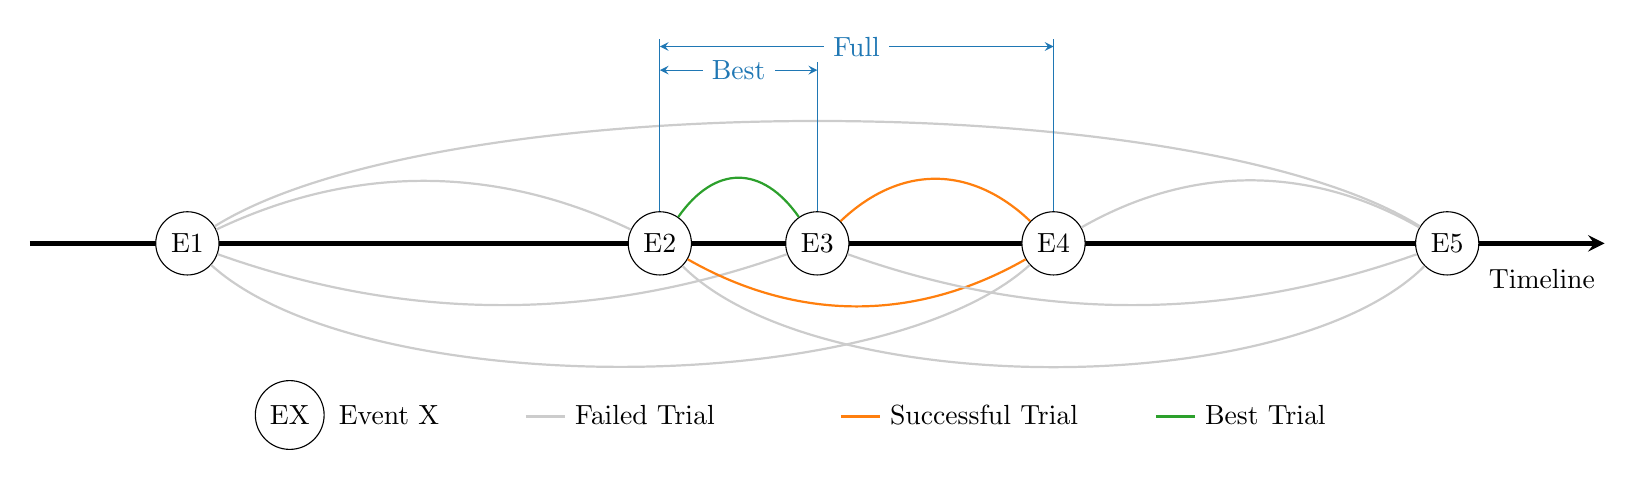
\begin{tikzpicture}
    \definecolor{C0}{HTML}{1f77b4}
    \definecolor{C1}{HTML}{ff7f0e}
    \definecolor{C2}{HTML}{2ca02c}
    \definecolor{C3}{HTML}{cccccc}

    \path[draw, ultra thick, -stealth] (0,0) -- (20,0);

    \node[draw, shape=circle, fill=white] (e1) at (2,0) {E1};
    \node[draw, shape=circle, fill=white] (e2) at (8,0) {E2};
    \node[draw, shape=circle, fill=white] (e3) at (10,0) {E3};
    \node[draw, shape=circle, fill=white] (e4) at (13,0) {E4};
    \node[draw, shape=circle, fill=white] (e5) at (18,0) {E5};

    \node at (20,-0.2) [anchor=north east] {Timeline};


    \path[draw=C3, thick] (e1) .. controls ($ (e1)!.35!(e2) + (0,1) $) and ($ (e1)!.65!(e2) + (0,1) $) .. (e2);
    \path[draw=C3, thick] (e1) .. controls ($ (e1)!.35!(e3) + (0,-1) $) and ($ (e1)!.65!(e3) + (0,-1) $) .. (e3);
    \path[draw=C3, thick] (e1) .. controls ($ (e1)!.20!(e4) + (0,-2) $) and ($ (e1)!.80!(e4) + (0,-2) $) .. (e4);
    \path[draw=C3, thick] (e1) .. controls ($ (e1)!.20!(e5) + (0,2) $) and ($ (e1)!.80!(e5) + (0,2) $) .. (e5);
    \path[draw=C2, thick] (e2) .. controls ($ (e2)!.35!(e3) + (0,1) $) and ($ (e2)!.65!(e3) + (0,1) $) .. (e3);
    \path[draw=C1, thick] (e2) .. controls ($ (e2)!.35!(e4) + (0,-1) $) and ($ (e2)!.65!(e4) + (0,-1) $) .. (e4);
    \path[draw=C3, thick] (e2) .. controls ($ (e2)!.20!(e5) + (0,-2) $) and ($ (e2)!.80!(e5) + (0,-2) $) .. (e5);
    \path[draw=C1, thick] (e3) .. controls ($ (e3)!.35!(e4) + (0,1) $) and ($ (e3)!.65!(e4) + (0,1) $) .. (e4);
    \path[draw=C3, thick] (e3) .. controls ($ (e3)!.35!(e5) + (0,-1) $) and ($ (e3)!.65!(e5) + (0,-1) $) .. (e5);
    \path[draw=C3, thick] (e4) .. controls ($ (e4)!.35!(e5) + (0,1) $) and ($ (e4)!.65!(e5) + (0,1) $) .. (e5);

    \path[draw=C0] (e2) -- ($ (e2) + (0,2.6) $);
    \path[draw=C0] (e3) -- ($ (e3) + (0,2.3) $);
    \path[draw=C0, stealth-stealth] ($ (e2) + (0,2.2) $) -- node [fill=white] {\textcolor{C0}{Best}} ($ (e3) + (0,2.2) $);
    \path[draw=C0] (e4) -- ($ (e4) + (0,2.6) $);
    \path[draw=C0, stealth-stealth] ($ (e2) + (0,2.5) $) -- node [fill=white] {\textcolor{C0}{Full}} ($ (e4) + (0,2.5) $);

    \begin{scope}[xshift=3.3cm, yshift=-2.3cm]
        \node[draw, shape=circle, anchor=base] (ex) at (0,0) {EX};
        \node at (0.5,0) [anchor=base west] {Event X};
        \path[draw=C3, thick] (3,0.1) -- (3.5,0.1);
        \node at (3.5,0) [right, anchor=base west] {Failed Trial};
        \path[draw=C1, thick] (7,0.1) -- (7.5,0.1);
        \node at (7.5,0) [right, anchor=base west] {Successful Trial};
        \path[draw=C2, thick] (11,0.1) -- (11.5,0.1);
        \node at (11.5,0) [right, anchor=base west] {Best Trial};
    \end{scope}


\end{tikzpicture}
\end{document}
